\documentclass[11pt]{article}

\usepackage[margin=1in]{geometry}
\usepackage[T1]{fontenc}
\usepackage{lmodern}
\usepackage{microtype}
\usepackage{amsmath,amssymb,amsthm,mathtools}
\usepackage{mathrsfs}
\usepackage[dvipsnames]{xcolor}
\usepackage[most]{tcolorbox}
\usepackage{graphicx}
\graphicspath{{figures/}{notes/figures/}}
\usepackage{tikz}
\usetikzlibrary{decorations.markings,patterns}
\usepackage{pgfplots}
\pgfplotsset{compat=1.17}
\usepackage{enumitem}
\usepackage{tocloft}
\usepackage[hidelinks]{hyperref}

\definecolor{courseblue}{HTML}{1F4E79}
\definecolor{lightblue}{HTML}{EAF2F8}
\definecolor{lightgreen}{HTML}{EAF7EA}
\definecolor{lightpink}{HTML}{FCE8EF}
\definecolor{lightyellow}{HTML}{FFF8D6}
\definecolor{warningyellow}{HTML}{D6A000}
\definecolor{exercisebg}{HTML}{FDEAEA}
\definecolor{exerciseframe}{HTML}{B54040}
\definecolor{examplebg}{HTML}{F4FAFE}
\definecolor{exampleframe}{HTML}{85C1E9}
\definecolor{darkgray}{HTML}{333333}
\definecolor{lightorange}{HTML}{FDEBD8}
\definecolor{orangeframe}{HTML}{E08A3C}
\definecolor{remarkbg}{HTML}{F3EEFB}
\definecolor{remarkframe}{HTML}{9B7FC9}
\definecolor{cayleyred}{HTML}{C0392B}
\definecolor{cayleygreen}{HTML}{1E8449}
\definecolor{cayleyblue}{HTML}{1F5FA0}
\definecolor{cayleyorange}{HTML}{D35400}
\definecolor{cayleypurple}{HTML}{7D3C98}
\definecolor{cayleyteal}{HTML}{117A65}

\setlength{\parindent}{0pt}
\setlength{\parskip}{0.45em}
\setlist[itemize]{topsep=0.25em,itemsep=0.15em}
\renewcommand{\cftsecleader}{\cftdotfill{\cftdotsep}}
\renewcommand{\cftsubsecleader}{\cftdotfill{\cftdotsep}}

\theoremstyle{plain}
\newtheorem{theorem}{Theorem}[section]
\newtheorem{proposition}[theorem]{Proposition}
\newtheorem{lemma}[theorem]{Lemma}
\newtheorem{corollary}[theorem]{Corollary}
\theoremstyle{definition}
\newtheorem{definition}[theorem]{Definition}
\newtheorem{example}[theorem]{Example}
\newtheorem{exercise}[theorem]{Exercise}
\newtheoremstyle{boldremark}
  {3pt}{3pt}{\normalfont}{}{\bfseries}{.}{.5em}
  {\thmname{#1}\thmnumber{ #2}\thmnote{ (#3)}}
\theoremstyle{boldremark}
\newtheorem*{remark}{Remark}
\theoremstyle{remark}
\newtheorem*{fact}{Fact}
\newtheorem*{warning}{Warning}

\tcolorboxenvironment{definition}{
  enhanced,
  unbreakable,
  colback=lightgreen,
  colframe=ForestGreen,
  boxrule=0.7pt,
  arc=2pt,
  left=6pt,
  right=6pt,
  top=5pt,
  bottom=5pt
}

\tcolorboxenvironment{remark}{
  enhanced,
  colback=remarkbg,
  colframe=remarkframe,
  before upper={\setlength{\parskip}{0.5em}},
  boxrule=0.7pt,
  arc=2pt,
  left=6pt,
  right=6pt,
  top=5pt,
  bottom=5pt
}

\tcolorboxenvironment{warning}{
  enhanced,
  colback=lightyellow,
  colframe=warningyellow,
  boxrule=0.7pt,
  arc=2pt,
  left=6pt,
  right=6pt,
  top=5pt,
  bottom=5pt
}

\tcolorboxenvironment{exercise}{
  enhanced,
  colback=exercisebg,
  colframe=exerciseframe,
  boxrule=1pt,
  arc=2pt,
  left=6pt,
  right=6pt,
  top=5pt,
  bottom=5pt
}

\tcolorboxenvironment{example}{
  enhanced,
  colback=examplebg,
  colframe=exampleframe,
  boxrule=0.7pt,
  arc=2pt,
  left=6pt,
  right=6pt,
  top=5pt,
  bottom=5pt
}

\numberwithin{equation}{section}

\newcommand{\be}{\begin{eqnarray}}
\newcommand{\ee}{\end{eqnarray}}
\newcommand{\C}{\mathbb{C}}
\newcommand{\R}{\mathbb{R}}
\newcommand{\N}{\mathbb{N}}
\newcommand{\Z}{\mathbb{Z}}
\DeclareMathOperator{\Log}{Log}
\DeclareMathOperator{\Arg}{Arg}

\DeclareMathOperator{\Hol}{\mathcal{H}\mathrm{ol}}
\DeclareMathOperator{\Real}{Re}
\DeclareMathOperator{\Imag}{Im}
\newcommand{\A}{\mathcal{A}}
\newcommand{\CT}{\C[[T]]}
\newcommand{\CLT}{\C((T))}
\tcbset{breakable}
% Compact spacing around diagrams; keep the main text at 11pt.
\newenvironment{lecturefigure}
 {\par\addvspace{0.25em}\begingroup\setlength{\parskip}{0pt}\centering}
 {\par\endgroup\addvspace{0.25em}}
\begin{document}

\begin{center}
  \colorbox{lightblue}{%
    \begin{minipage}{0.94\textwidth}
      \vspace{0.55em}
      \begin{tabular*}{\textwidth}{@{\extracolsep{\fill}}lr}
        {\color{courseblue}\bfseries\LARGE Lecture 30} &
        {\color{courseblue}\bfseries\LARGE MATH 411}\\[0.35em]
        \textbf{Fall 2026} & \textbf{Date: Nov 27, 2026}\\
        & \textbf{Instructor: Manish Patnaik}
      \end{tabular*}
      \vspace{0.45em}
    \end{minipage}}
\end{center}

\setcounter{tocdepth}{1}
\tableofcontents
\vspace{0.45em}

% Moved from Lecture 29, Sections 3--4 (handwritten Lecture 28, Nov. 25).
\section{Contour shifting and exponential decay}

Recall from Lecture~29 that for a function $f$ on $\R$ of moderate decay,
its Fourier transform is defined by
\[
 \widehat f(\xi) = \int_{-\infty}^{\infty} f(x)e^{-2\pi i x\xi}\,dx,
 \qquad \xi\in\R.
\]
For $a>0$, the class $\mathcal F_a$ consists of all functions $f$
holomorphic on the open horizontal strip
$S_a=\{z\in\C:|\Imag z|<a\}$ for which there exists a single constant
$A>0$ satisfying the uniform moderate decay bound
\[
 |f(x+iy)|\leq\frac{A}{1+x^2}\qquad(x\in\R,\ |y|<a),
\]
and $\mathcal F=\bigcup_{a>0}\mathcal F_a$. We now show that holomorphicity
on the strip $S_a$ translates directly into exponential decay of
$\widehat f(\xi)$ as $|\xi|\to\infty$.

\begin{theorem}[Shifting the Fourier integral]\label{thm:shift}
Let $f\in\mathcal F_a$ with constant $A$. For $|y|<a$ and $\xi\in\R$,
\begin{equation}\label{eq:shift}
 \widehat f(\xi)=\int_{-\infty}^{\infty}
 f(x+iy)e^{-2\pi i(x+iy)\xi}\,dx .
\end{equation}
In particular, for $0\leq b<a$,
\begin{equation}\label{eq:exp-decay}
 |\widehat f(\xi)|\leq\pi A e^{-2\pi b|\xi|}.
\end{equation}
\end{theorem}

\begin{lecturefigure}
\begin{minipage}{\linewidth}\centering
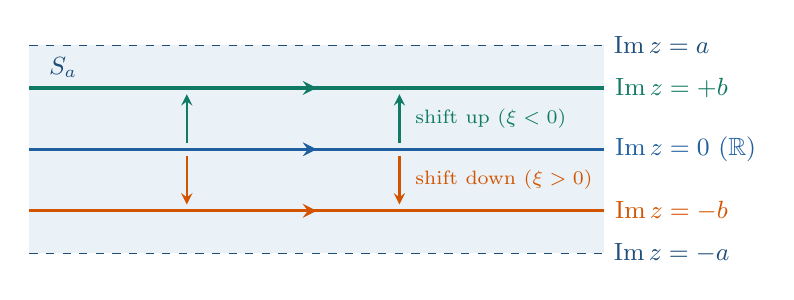
\begin{tikzpicture}[>=stealth,font=\small,
 midarrow/.style={postaction={decorate},decoration={markings,mark=at position .50 with {\arrow{>}}}}]
 % Holomorphic strip S_a
 \fill[lightblue] (-3.65,-1.32) rectangle (3.65,1.32);
 \draw[courseblue,dashed] (-3.65,1.32) -- (3.65,1.32) node[right,text=courseblue] {$\Imag z=a$};
 \draw[courseblue,dashed] (-3.65,-1.32) -- (3.65,-1.32) node[right,text=courseblue] {$\Imag z=-a$};
 \node[text=courseblue] at (-3.22,1.04) {$S_a$};
 % Original contour: real line
 \draw[cayleyblue,very thick,midarrow] (-3.65,0) -- (3.65,0) node[right,text=cayleyblue] {$\Imag z=0$ ($\R$)};
 % Shifted contour up: Im z = +b (for xi < 0)
 \draw[cayleyteal,very thick,midarrow] (-3.65,0.78) -- (3.65,0.78) node[right,text=cayleyteal] {$\Imag z=+b$};
 % Shifted contour down: Im z = -b (for xi > 0)
 \draw[cayleyorange,very thick,midarrow] (-3.65,-0.78) -- (3.65,-0.78) node[right,text=cayleyorange] {$\Imag z=-b$};
 % Vertical shift arrows
 \draw[->,cayleyteal,thick] (-1.65,0.08) -- (-1.65,0.70);
 \draw[->,cayleyteal,thick] (1.05,0.08) -- (1.05,0.70)
  node[midway,right,xshift=2pt,font=\scriptsize,text=cayleyteal] {shift up ($\xi<0$)};
 \draw[->,cayleyorange,thick] (-1.65,-0.08) -- (-1.65,-0.70);
 \draw[->,cayleyorange,thick] (1.05,-0.08) -- (1.05,-0.70)
  node[midway,right,xshift=2pt,font=\scriptsize,text=cayleyorange] {shift down ($\xi>0$)};
\end{tikzpicture}

\vspace{0.15em}
{\small The line of integration $\R$ (blue) can be shifted vertically to any
height $y\in(-a,a)$ inside $S_a$ without changing $\widehat f(\xi)$. Shifting
down to $-b$ for $\xi>0$ (orange) or up to $+b$ for $\xi<0$ (teal) yields
the exponential decay factor $|e^{-2\pi i(x+iy)\xi}|=e^{-2\pi b|\xi|}$.}
\end{minipage}
\end{lecturefigure}

\begin{proof}
For fixed $\xi\in\R$, the function $g(z)=f(z)e^{-2\pi i z\xi}$ is
holomorphic on $S_a$. Take the rectangle with horizontal edges at
heights $0$ and $y$ and vertical edges at $x=\pm R$. By Cauchy's theorem,
the integral around this rectangle vanishes.

\begin{lecturefigure}
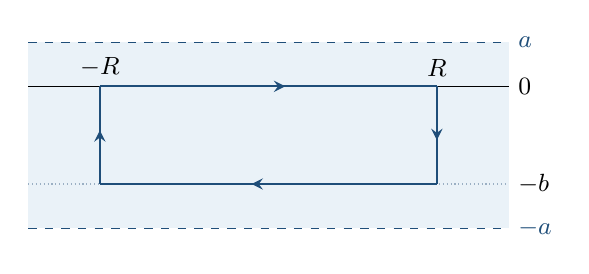
\begin{tikzpicture}[>=stealth,font=\small,
 midarrow/.style={postaction={decorate},decoration={markings,mark=at position .55 with {\arrow{>}}}}]
 \fill[lightblue] (-3.05,-1.28) rectangle (3.05,1.08);
 \draw[courseblue,dashed] (-3.05,1.08) -- (3.05,1.08) node[right] {$a$};
 \draw[courseblue,dashed] (-3.05,-1.28) -- (3.05,-1.28) node[right] {$-a$};
 \draw (-3.05,0.52) -- (3.05,0.52) node[right] {$0$};
 \draw[courseblue!45,densely dotted] (-3.05,-0.72) -- (3.05,-0.72) node[right,text=black] {$-b$};
 \draw[courseblue,thick,midarrow] (-2.14,0.52) -- (2.14,0.52);
 \draw[courseblue,thick,midarrow] (2.14,0.52) -- (2.14,-0.72);
 \draw[courseblue,thick,midarrow] (2.14,-0.72) -- (-2.14,-0.72);
 \draw[courseblue,thick,midarrow] (-2.14,-0.72) -- (-2.14,0.52);
 \node[above] at (-2.14,0.52) {$-R$}; \node[above] at (2.14,0.52) {$R$};
\end{tikzpicture}

{\small The rectangular contour for a downward shift to $y=-b$.}
\end{lecturefigure}

For $y<0$ (as shown above for $y=-b$), traversing the rectangle clockwise
orients the top edge along $\R$ from left to right and the bottom edge at
height $y$ from right to left:
\[
 \int_{\text{top}} g(z)\,dz
  = \int_{-R}^{R} f(x)e^{-2\pi ix\xi}\,dx,
 \qquad
 \int_{\text{bottom}} g(z)\,dz
  = -\int_{-R}^{R} f(x+iy)e^{-2\pi i(x+iy)\xi}\,dx.
\]
(When $y>0$, the roles of the top and bottom edges reverse, and traversing
counterclockwise produces the same two horizontal integrals with the same
signs.) Cauchy's theorem therefore gives
\[
 \int_{-R}^{R} f(x)e^{-2\pi ix\xi}\,dx
 - \int_{-R}^{R} f(x+iy)e^{-2\pi i(x+iy)\xi}\,dx
 + \int_{\text{vertical edges}} g(z)\,dz = 0.
\]

Along either vertical edge $z=\pm R+it$ between heights $0$ and $y$,
\[
 |g(z)|\leq\frac{A}{1+R^2}e^{2\pi|y\xi|}.
\]
The length of each edge is $|y|$, so both vertical integrals have modulus at
most $|y|A e^{2\pi|y\xi|}/(1+R^2)$ and tend to zero as $R\to\infty$. Both
horizontal integrals converge absolutely by moderate decay, so letting
$R\to\infty$ gives \eqref{eq:shift}.

Finally, for $\xi>0$ set $y=-b$, and for $\xi<0$ set $y=b$. In either case
\[
 \bigl|e^{-2\pi i(x+iy)\xi}\bigr| = e^{2\pi y\xi} = e^{-2\pi b|\xi|},
\]
so moving the absolute value inside \eqref{eq:shift} gives
\[
 |\widehat f(\xi)|
 \leq e^{-2\pi b|\xi|}\int_{-\infty}^{\infty}\frac{A}{1+x^2}\,dx
 = \pi A e^{-2\pi b|\xi|}.
\]
The same bound holds at $\xi=0$ and for $b=0$ by direct integration on the
real axis.
\end{proof}


\section{Fourier inversion}

The exponential decay bound \eqref{eq:exp-decay} ensures that $\widehat f$
is integrable on $\R$, so we can integrate $\widehat f(\xi)e^{2\pi i x\xi}$
over all frequencies $\xi$ and recover $f(x)$.

\begin{theorem}[Fourier inversion on $\mathcal F$]\label{thm:fourier-inversion}
If $f\in\mathcal F$, then for every $x\in\R$,
\begin{equation}\label{eq:fourier-inversion}
 \boxed{\displaystyle
  f(x)=\int_{-\infty}^{\infty}\widehat f(\xi)e^{2\pi ix\xi}\,d\xi.}
\end{equation}
The integral on the right converges absolutely.
\end{theorem}

We need one elementary integral before proving the theorem.

\begin{exercise}[An exponential integral]\label{ex:exp-integral}
For $A>0$ and $B\in\R$, verify directly (by integrating over $[0,T]$ and
letting $T\to\infty$) that
\[
 \int_0^\infty e^{-(A+iB)\xi}\,d\xi = \frac{1}{A+iB}.
\]
\end{exercise}

\begin{proof}[Proof of Theorem~\ref{thm:fourier-inversion}]
Choose $a>0$ with $f\in\mathcal F_a$ (with moderate decay constant $A$) and
fix $0<b<a$. By Theorem~\ref{thm:shift}, $|\widehat f(\xi)|\leq\pi A e^{-2\pi b|\xi|}$,
so $\widehat f$ is absolutely integrable on $\R$ and the inversion integral
converges absolutely. Split the integral at $\xi=0$:
\[
 \int_{-\infty}^{\infty}\widehat f(\xi)e^{2\pi ix\xi}\,d\xi
 = \int_{-\infty}^{0}\widehat f(\xi)e^{2\pi ix\xi}\,d\xi
 + \int_{0}^{\infty}\widehat f(\xi)e^{2\pi ix\xi}\,d\xi.
\]

\textbf{The positive half ($\xi\geq 0$).} By Theorem~\ref{thm:shift}, shift
the line of integration in $\widehat f(\xi)$ downward to height $-b$:
\[
 \widehat f(\xi) = \int_{-\infty}^{\infty} f(u-ib)e^{-2\pi i(u-ib)\xi}\,du.
\]
Substituting this into the integral over $[0,\infty)$ yields the double
integral
\[
 \int_0^\infty \widehat f(\xi)e^{2\pi ix\xi}\,d\xi
 = \int_0^\infty\left(\int_{-\infty}^{\infty}
    f(u-ib)e^{-2\pi i(u-ib-x)\xi}\,du\right)d\xi.
\]
For $u\in\R$ and $\xi\geq 0$, the integrand satisfies
\[
 \bigl|f(u-ib)e^{-2\pi i(u-ib-x)\xi}\bigr|
 = |f(u-ib)|\,e^{-2\pi b\xi}
 \leq \frac{A}{1+u^2}\,e^{-2\pi b\xi},
\]
whose double integral over $\R\times[0,\infty)$ is finite (equal to
$\frac{A}{2b}$). Hence Fubini's theorem permits us to interchange the order
of integration:
\begin{align*}
 \int_0^\infty\widehat f(\xi)e^{2\pi ix\xi}\,d\xi
 &= \int_{-\infty}^{\infty} f(u-ib)
    \left(\int_0^\infty e^{-2\pi i(u-ib-x)\xi}\,d\xi\right)du \\
 &= \int_{-\infty}^{\infty} f(u-ib)
    \left(\int_0^\infty e^{-\bigl(2\pi b+2\pi i(u-x)\bigr)\xi}\,d\xi\right)du.
\end{align*}
Applying Exercise~\ref{ex:exp-integral} with $2\pi b>0$ and $2\pi(u-x)\in\R$
evaluates the inner integral as
\[
 \frac{1}{2\pi b+2\pi i(u-x)} = \frac{1}{2\pi i(u-ib-x)}.
\]
Therefore, writing $L_-=\{u-ib:u\in\R\}$ oriented from left to right,
\begin{equation}\label{eq:inv-pos}
 \int_0^\infty\widehat f(\xi)e^{2\pi ix\xi}\,d\xi
 = \frac{1}{2\pi i}\int_{-\infty}^{\infty}\frac{f(u-ib)}{u-ib-x}\,du
 = \frac{1}{2\pi i}\int_{L_-}\frac{f(z)}{z-x}\,dz.
\end{equation}

\textbf{The negative half ($\xi\leq 0$).} Shift the contour defining
$\widehat f(\xi)$ upward to height $+b$ and substitute $\xi=-\eta$
($\eta\geq 0$). The exponent becomes
\[
 -2\pi i(u+ib-x)(-\eta)
 = 2\pi i(u+ib-x)\eta
 = -\bigl(2\pi b-2\pi i(u-x)\bigr)\eta,
\]
so the integrand again has modulus bounded by $\frac{A}{1+u^2}e^{-2\pi b\eta}$.
By Fubini's theorem and Exercise~\ref{ex:exp-integral},
\begin{align*}
 \int_{-\infty}^0\widehat f(\xi)e^{2\pi ix\xi}\,d\xi
 &= \int_{-\infty}^{\infty} f(u+ib)
    \left(\int_0^\infty e^{-\bigl(2\pi b-2\pi i(u-x)\bigr)\eta}\,d\eta\right)du \\
 &= \int_{-\infty}^{\infty}\frac{f(u+ib)}{2\pi b-2\pi i(u-x)}\,du
  = -\frac{1}{2\pi i}\int_{-\infty}^{\infty}\frac{f(u+ib)}{u+ib-x}\,du.
\end{align*}
Writing $L_+=\{u+ib:u\in\R\}$ oriented from left to right, this reads
\begin{equation}\label{eq:inv-neg}
 \int_{-\infty}^0\widehat f(\xi)e^{2\pi ix\xi}\,d\xi
 = -\frac{1}{2\pi i}\int_{L_+}\frac{f(z)}{z-x}\,dz.
\end{equation}

\textbf{Closing the contour.} For $R>|x|$, let $\gamma_R$ be the
counterclockwise boundary of the rectangle with vertices $\pm R\pm ib$. Its
bottom edge traverses $L_-$ from left to right, and its top edge traverses
$L_+$ from right to left.

\begin{lecturefigure}
\begin{minipage}{\linewidth}\centering
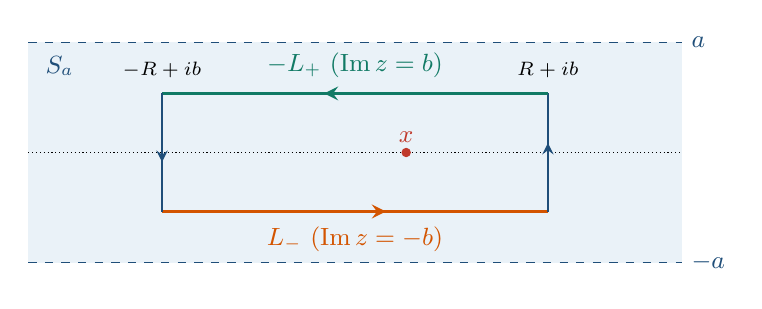
\begin{tikzpicture}[>=stealth,font=\small,
 midarrow/.style={postaction={decorate},decoration={markings,mark=at position .58 with {\arrow{>}}}}]
 \fill[lightblue] (-4.15,-1.40) rectangle (4.15,1.40);
 \draw[courseblue,dashed] (-4.15,1.40) -- (4.15,1.40) node[right,text=courseblue] {$a$};
 \draw[courseblue,dashed] (-4.15,-1.40) -- (4.15,-1.40) node[right,text=courseblue] {$-a$};
 \node[text=courseblue] at (-3.75,1.10) {$S_a$};
 \draw[densely dotted] (-4.15,0) -- (4.15,0);
 \draw[cayleyorange,very thick,midarrow] (-2.45,-0.75) -- (2.45,-0.75);
 \draw[courseblue,thick,midarrow] (2.45,-0.75) -- (2.45,0.75);
 \draw[cayleyteal,very thick,midarrow] (2.45,0.75) -- (-2.45,0.75);
 \draw[courseblue,thick,midarrow] (-2.45,0.75) -- (-2.45,-0.75);
 \node[above,yshift=2pt,text=cayleyteal] at (0,0.75) {$-L_+$ ($\Imag z=b$)};
 \node[below,yshift=-2pt,text=cayleyorange] at (0,-0.75) {$L_-$ ($\Imag z=-b$)};
 \node[above,yshift=2pt,font=\scriptsize] at (-2.45,0.75) {$-R+ib$};
 \node[above,yshift=2pt,font=\scriptsize] at (2.45,0.75) {$R+ib$};
 \fill[cayleyred] (0.65,0) circle (1.7pt) node[above,text=cayleyred] {$x$};
\end{tikzpicture}

\vspace{0.15em}
{\small Closing the two shifted horizontal lines at $\pm R$ encloses the
single simple pole of $f(z)/(z-x)$ at $z=x$.}
\end{minipage}
\end{lecturefigure}

Inside $\gamma_R$, the function $z\mapsto f(z)/(z-x)$ has at most a simple
pole at $z=x$ with residue $f(x)$, so by the residue theorem (or Cauchy's
integral formula),
\[
 f(x) = \frac{1}{2\pi i}\int_{\gamma_R}\frac{f(z)}{z-x}\,dz.
\]
Along either vertical side $z=\pm R+iy$ ($-b\leq y\leq b$), we have
$|z-x|\geq|\Real z-x|\geq R-|x|$ and $|f(z)|\leq A/(1+R^2)$, while the
edge has length $2b$. By the ML estimate, each vertical integral is bounded
by
\[
 \left|\int_{\text{vertical side}}\frac{f(z)}{z-x}\,dz\right|
 \leq \frac{2bA}{(1+R^2)(R-|x|)} \xrightarrow[R\to\infty]{} 0.
\]
Both horizontal integrals converge absolutely on $\R$ because
$|f(u\pm ib)/(u\pm ib-x)|\leq \frac{A}{b(1+u^2)}$. Letting $R\to\infty$
and combining with \eqref{eq:inv-pos} and \eqref{eq:inv-neg}, we conclude
that
\begin{align*}
 f(x)
 &= \frac{1}{2\pi i}\int_{L_-}\frac{f(z)}{z-x}\,dz
  - \frac{1}{2\pi i}\int_{L_+}\frac{f(z)}{z-x}\,dz \\
 &= \int_0^\infty\widehat f(\xi)e^{2\pi ix\xi}\,d\xi
  + \int_{-\infty}^0\widehat f(\xi)e^{2\pi ix\xi}\,d\xi
  = \int_{-\infty}^{\infty}\widehat f(\xi)e^{2\pi ix\xi}\,d\xi. \qedhere
\end{align*}
\end{proof}


% Source: handwritten Lecture 29, Nov. 29, pp. 1--4.
\section{The Poisson summation formula}

In the proof of Fourier inversion, integrating $f(z)/(z-x)$ around a
rectangle in $S_a$ picked out the value $f(x)$ at a single point $x\in\R$.
If we replace the kernel $1/(z-x)$ by a meromorphic function with simple
poles at \emph{every} integer $n\in\Z$, the same contour-shifting technique
produces a remarkable identity relating the sums of $f$ and $\widehat f$
over the integers.

\begin{theorem}[Poisson summation formula]\label{thm:poisson-summation}
Let $f\in\mathcal F_a$ for some $a>0$. Then
\begin{equation}\label{eq:poisson}
 \boxed{\displaystyle
  \sum_{n\in\Z} f(n) = \sum_{n\in\Z}\widehat f(n).}
\end{equation}
Both series converge absolutely.
\end{theorem}

\begin{proof}
Fix $0<b<a$ and consider the function
\[
 Q(z) = \frac{f(z)}{e^{2\pi i z}-1}
\]
on the strip $S_a$.

\textbf{Step 1: Poles and residues.}
The denominator $h(z)=e^{2\pi i z}-1$ is entire and vanishes if and only if
$e^{2\pi i z}=1$, i.e., $z\in\Z$. At each integer $n\in\Z$,
\[
 h'(n) = 2\pi i e^{2\pi i n} = 2\pi i \neq 0,
\]
so every $n\in\Z$ is a simple zero of $h$. Hence $\frac{1}{e^{2\pi iz}-1}$
is meromorphic on $\C$ with simple poles at $0,\pm 1,\pm 2,\dots$, and
$Q(z)$ is meromorphic on $S_a$ with residue at $z=n$ given by
\[
 \operatorname{Res}_{z=n}\frac{f(z)}{e^{2\pi i z}-1}
 = \frac{f(n)}{h'(n)} = \frac{f(n)}{2\pi i}
\]
(which also holds as $0$ when $f(n)=0$ and the singularity is removable).

\textbf{Step 2: Residue theorem on a rectangle $\gamma_N$.}
For each integer $N\geq 1$, set $R_N=N+\tfrac12$, and let $\gamma_N$ be the
counterclockwise boundary of the rectangle with vertices $\pm R_N\pm ib$.
Since $0<b<a$, the rectangle lies strictly inside $S_a$. Because
$R_N=N+\tfrac12$ is a half-integer, the vertical sides avoid the poles at
$\Z$, and the integers inside $\gamma_N$ are precisely
$-N,\dots,-1,0,1,\dots,N$.

\begin{lecturefigure}
\begin{minipage}{\linewidth}\centering
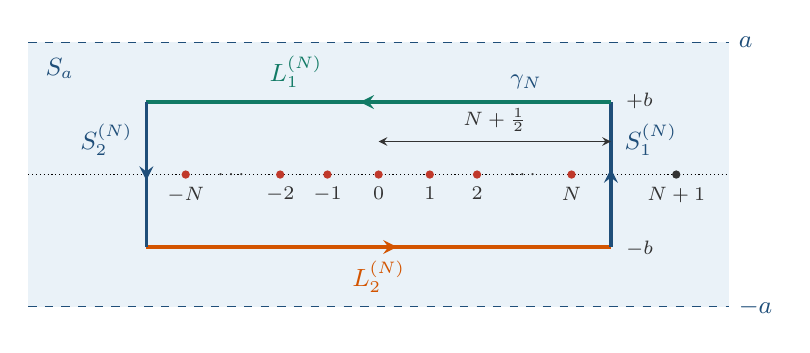
\begin{tikzpicture}[>=stealth,font=\small,
 midarrow/.style={postaction={decorate},decoration={markings,mark=at position .54 with {\arrow{>}}}}]
 % Strip S_a
 \fill[lightblue] (-4.45,-1.68) rectangle (4.45,1.68);
 \draw[courseblue,dashed] (-4.45,1.68) -- (4.45,1.68) node[right,text=courseblue] {$a$};
 \draw[courseblue,dashed] (-4.45,-1.68) -- (4.45,-1.68) node[right,text=courseblue] {$-a$};
 \node[text=courseblue] at (-4.05,1.35) {$S_a$};
 % Real axis
 \draw[densely dotted] (-4.45,0) -- (4.45,0);
 % Rectangle gamma_N
 \draw[cayleyorange,very thick,midarrow] (-2.95,-0.92) -- (2.95,-0.92);
 \draw[courseblue,very thick,midarrow] (2.95,-0.92) -- (2.95,0.92);
 \draw[cayleyteal,very thick,midarrow] (2.95,0.92) -- (-2.95,0.92);
 \draw[courseblue,very thick,midarrow] (-2.95,0.92) -- (-2.95,-0.92);
 % Integer poles inside and N+1 outside
 \foreach \x/\lab in {-2.45/-N,-1.25/-2,-0.65/-1,0/0,0.65/1,1.25/2,2.45/N} {
  \fill[cayleyred] (\x,0) circle (1.5pt);
  \node[below,font=\scriptsize,text=darkgray] at (\x,-0.04) {$\lab$};
 }
 \node[font=\scriptsize,text=darkgray] at (-1.85,0) {$\cdots$};
 \node[font=\scriptsize,text=darkgray] at (1.85,0) {$\cdots$};
 \fill[darkgray] (3.78,0) circle (1.5pt);
 \node[below,font=\scriptsize,text=darkgray] at (3.78,-0.04) {$N+1$};
 % Half-width indicator N + 1/2
 \draw[<->,darkgray,thin] (0,0.42) -- (2.95,0.42)
  node[midway,above,font=\scriptsize,text=darkgray] {$N+\tfrac12$};
 % Labels for edges and heights
 \node[above,yshift=1pt,text=cayleyteal] at (-1.05,0.94) {$L_1^{(N)}$};
 \node[below,yshift=-1pt,text=cayleyorange] at (0,-0.94) {$L_2^{(N)}$};
 \node[right,text=courseblue] at (3.00,0.44) {$S_1^{(N)}$};
 \node[left,text=courseblue] at (-3.00,0.44) {$S_2^{(N)}$};
 \node[right,font=\scriptsize,text=darkgray] at (3.02,0.94) {$+b$};
 \node[right,font=\scriptsize,text=darkgray] at (3.02,-0.94) {$-b$};
 \node[above right,font=\footnotesize,text=courseblue] at (1.55,0.96) {$\gamma_N$};
\end{tikzpicture}

\vspace{0.15em}
{\small The counterclockwise rectangular contour $\gamma_N$ inside $S_a$,
with horizontal edges at $\Imag z=\pm b$ and vertical edges at
$\Real z=\pm(N+\tfrac12)$, encloses the poles at $-N,\dots,N$.}
\end{minipage}
\end{lecturefigure}

Applying the residue theorem to $Q$ on $\gamma_N$ gives
\[
 \frac{1}{2\pi i}\int_{\gamma_N}\frac{f(z)}{e^{2\pi i z}-1}\,dz
 = \sum_{|n|\leq N}\frac{f(n)}{2\pi i},
\]
and therefore
\begin{equation}\label{eq:poisson-rect}
 \sum_{|n|\leq N} f(n) = \int_{\gamma_N}\frac{f(z)}{e^{2\pi i z}-1}\,dz.
\end{equation}
As $N\to\infty$, the left-hand side converges absolutely to
$\sum_{n\in\Z} f(n)$, because moderate decay gives
$|f(n)|\leq A/(1+n^2)$ and $\sum_{n\in\Z}(1+n^2)^{-1}<\infty$.

\textbf{Step 3: Decomposing $\gamma_N$ and estimating the vertical sides.}
Write the integral around $\gamma_N$ as the sum over its four oriented edges:
\[
 \int_{\gamma_N} Q(z)\,dz
 = \int_{L_1^{(N)}} Q(z)\,dz
 + \int_{L_2^{(N)}} Q(z)\,dz
 + \int_{S_1^{(N)}} Q(z)\,dz
 + \int_{S_2^{(N)}} Q(z)\,dz,
\]
where $L_2^{(N)}$ is the bottom segment $z(t)=t-ib$ for $t\in[-R_N,R_N]$
(oriented left to right), $L_1^{(N)}$ is the top segment oriented right to
left (so $-L_1^{(N)}$ is parametrized by $z(t)=t+ib$ for $t\in[-R_N,R_N]$),
and $S_1^{(N)},S_2^{(N)}$ are the right and left vertical segments at
$x=\pm R_N$.

To see why the vertical integrals vanish as $N\to\infty$, write $z=x+iy$
and note that
\[
 e^{2\pi i(x+iy)}-1 = e^{2\pi i x}e^{-2\pi y}-1.
\]
On $S_1^{(N)}$ and $S_2^{(N)}$ we have $x=\pm(N+\tfrac12)$ (not an integer!),
so $e^{2\pi i x}=e^{\pm i\pi}=-1$, and hence
\[
 e^{2\pi i z}-1 = -e^{-2\pi y}-1 = -(1+e^{-2\pi y}).
\]
In particular, $|e^{2\pi i z}-1|=1+e^{-2\pi y}\geq 1$ on both vertical
sides, so the denominator stays bounded away from $0$ uniformly in $N$ and
$y\in[-b,b]$. Combining this with $|f(\pm R_N+iy)|\leq A/(1+R_N^2)$ and the
edge length $2b$, the ML estimate gives
\[
 \left|\int_{S_j^{(N)}}\frac{f(z)}{e^{2\pi i z}-1}\,dz\right|
 \leq \frac{2bA}{1+(N+\tfrac12)^2} \xrightarrow[N\to\infty]{} 0
 \qquad (j=1,2).
\]

\textbf{Step 4: Passing to the infinite horizontal lines.}
Let $L_2=\{x-ib:x\in\R\}$ oriented left to right, and let
$L_1=\{x+ib:x\in\R\}$ oriented right to left. On $L_2$,
$|e^{2\pi i(x-ib)}|=e^{2\pi b}>1$, so $|e^{2\pi i z}-1|\geq e^{2\pi b}-1>0$;
on $L_1$, $|e^{2\pi i(x+ib)}|=e^{-2\pi b}<1$, so
$|e^{2\pi i z}-1|\geq 1-e^{-2\pi b}>0$. Since $|f(x\pm ib)|\leq A/(1+x^2)$
is integrable on $\R$, both horizontal integrals converge absolutely as
$N\to\infty$. Taking $N\to\infty$ in \eqref{eq:poisson-rect} therefore gives
\begin{equation}\label{eq:poisson-lines}
 \sum_{n\in\Z} f(n)
 = \int_{L_1}\frac{f(z)}{e^{2\pi i z}-1}\,dz
 + \int_{L_2}\frac{f(z)}{e^{2\pi i z}-1}\,dz.
\end{equation}

\textbf{Step 5: Geometric series on $L_2$ (positive frequencies).}
For any complex number $w$ with $|w|>1$,
\[
 \frac{1}{w-1}
 = \frac{w^{-1}}{1-w^{-1}}
 = w^{-1}\sum_{k=0}^{\infty} w^{-k}
 = \sum_{n=1}^{\infty} w^{-n}.
\]
On $L_2$, we have $z=x-ib$ with $b>0$, so
$w=e^{2\pi i z}=e^{2\pi i x}e^{2\pi b}$ has $|w|=e^{2\pi b}>1$. Thus
\[
 \frac{1}{e^{2\pi i z}-1}
 = e^{-2\pi i z}\sum_{k=0}^{\infty} e^{-2\pi i k z}
 = \sum_{n=1}^{\infty} e^{-2\pi i n z}.
\]
To justify integrating term by term, note that for each $M\geq 1$ and
$z=x-ib\in L_2$, the geometric-series remainder satisfies
\[
 \left|\frac{1}{e^{2\pi i z}-1}-\sum_{n=1}^{M} e^{-2\pi i n z}\right|
 = \left|\frac{e^{-2\pi i(M+1)z}}{1-e^{-2\pi i z}}\right|
 \leq \frac{e^{-2\pi(M+1)b}}{1-e^{-2\pi b}}.
\]
Multiplying by $|f(x-ib)|\leq A/(1+x^2)$ and integrating over $x\in\R$
bounds the tail error by $\frac{\pi A e^{-2\pi(M+1)b}}{1-e^{-2\pi b}}\to 0$
as $M\to\infty$. We may therefore interchange the sum and integral, and by
Theorem~\ref{thm:shift} (shifting the line of integration in the definition
of $\widehat f(n)$ down to $L_2$),
\begin{align*}
 \int_{L_2}\frac{f(z)}{e^{2\pi i z}-1}\,dz
 &= \sum_{n=1}^{\infty}\int_{L_2} f(z)e^{-2\pi i n z}\,dz \\
 &= \sum_{n=1}^{\infty}\int_{-\infty}^{\infty}
    f(x-ib)e^{-2\pi i n(x-ib)}\,dx
  = \sum_{n=1}^{\infty}\widehat f(n).
\end{align*}

\textbf{Step 6: Geometric series on $L_1$ (nonpositive frequencies).}
For $|w|<1$, we instead expand
\[
 \frac{1}{w-1} = -\frac{1}{1-w} = -\sum_{m=0}^{\infty} w^m.
\]
On $L_1$, we have $z=x+ib$ with $b>0$, so
$w=e^{2\pi i z}=e^{2\pi i x}e^{-2\pi b}$ satisfies $|w|=e^{-2\pi b}<1$,
giving
\[
 \frac{1}{e^{2\pi i z}-1} = -\sum_{m=0}^{\infty} e^{2\pi i m z}.
\]
Because $L_1$ is oriented from right to left (opposite to $x\mapsto x+ib$),
reversing the orientation cancels the minus sign:
\[
 \int_{L_1}\frac{f(z)}{e^{2\pi i z}-1}\,dz
 = -\int_{-\infty}^{\infty}\frac{f(x+ib)}{e^{2\pi i(x+ib)}-1}\,dx
 = \int_{-\infty}^{\infty} f(x+ib)
    \sum_{m=0}^{\infty} e^{2\pi i m(x+ib)}\,dx.
\]
The same tail estimate ($\leq \frac{\pi A e^{-2\pi(M+1)b}}{1-e^{-2\pi b}}\to 0$)
justifies term-by-term integration, and applying Theorem~\ref{thm:shift}
with the contour shifted up to height $+b$ gives
\begin{align*}
 \int_{L_1}\frac{f(z)}{e^{2\pi i z}-1}\,dz
 &= \sum_{m=0}^{\infty}\int_{-\infty}^{\infty}
    f(x+ib)e^{-2\pi i(-m)(x+ib)}\,dx \\
 &= \sum_{m=0}^{\infty}\widehat f(-m)
  = \sum_{n=-\infty}^{0}\widehat f(n).
\end{align*}

\textbf{Step 7: Conclusion.}
Substituting the evaluations over $L_1$ and $L_2$ into
\eqref{eq:poisson-lines} yields
\[
 \sum_{n\in\Z} f(n)
 = \sum_{n=-\infty}^{0}\widehat f(n) + \sum_{n=1}^{\infty}\widehat f(n)
 = \sum_{n\in\Z}\widehat f(n).
\]
Finally, by Theorem~\ref{thm:shift} we have
$|\widehat f(n)|\leq \pi A e^{-2\pi b|n|}$, so $\sum_{n\in\Z}\widehat f(n)$
also converges absolutely.
\end{proof}

% Section 4 (Gaussian summation and theta inversion) moved to Lecture 31.

\end{document}
